\chapter{Conversion from \protect\LaTeX\ to HTML}
\label{ch:latex-to-html}

\section{Choosing your preferred workflow}

There are several tools available to perform conversion of \LaTeX\ to HTML. Here, we focus on \href{https://vlmantova.github.io/bookml/}{BookML}, which uses \href{https://math.nist.gov/~BMiller/LaTeXML/}{LaTeXML} in the background; note that this is the same technology used by \href{https://info.arxiv.org/about/accessible_HTML.html}{arXiv} to produce HTML versions of research papers from the \verb|.tex| source.

There are three steps to generating HTML notes from \LaTeX using BookML:

\begin{enumerate}
    \item write notes in \LaTeX{}, optionally using the School template;
    \item use BookML to convert \LaTeX{} code to HTML;
    \item share the HTML version with students.
\end{enumerate}

Your precise workflow will depend on how you wish to share the HTML version with students, whether you prefer to work in Overleaf or write \LaTeX{} locally, and whether you prefer the HTML conversion to be dealt with in the cloud (via GitHub) or on your local machine (via Docker). Some possible workflows are summarised in the figure below.

\begin{figure}[h]
    \centering
    \iflatexml
        
\includegraphics{img/process.svg}
    \else
        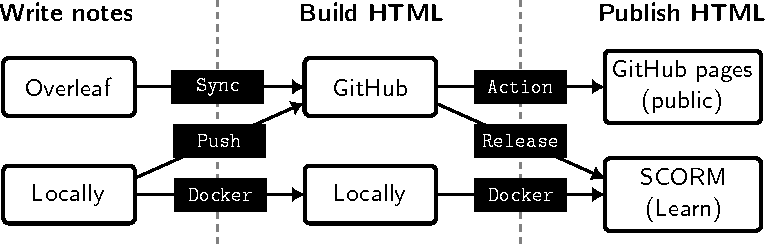
\includegraphics{img/process.pdf}
    \fi
    \caption{Workflow options to build HTML course materials.}
    \alttext{Flowchart showing different workflow options to build HTML course materials.}
    \label{fig:workflow}
\end{figure}

We give detailed guidance for two of these workflows: one with cloud-based conversion and one with local conversion. You can mix-and-match or deviate from these documented workflows if you feel comfortable doing so. If you're not sure where to start, cloud-based is easiest (Section~\ref{sec:github}).


\section{Cloud-based workflow (via GitHub)}
\label{sec:github}

The simplest way to generate HTML course materials makes use of GitHub to perform the conversion in the cloud, which means that you will not need to install anything on your computer. All you need to do is upload your \LaTeX{} source code to a (private) GitHub repository; the conversion to HTML is then done automatically.

Additionally, if you use Overleaf, you can set it up to connect to GitHub. After the initial setup, there will be no need to interact directly with GitHub. Here, we explain this particular workflow\footnote{You should also follow this section if you don't plan to use Overleaf, but still want to use the cloud-based conversion to HTML. The instructions will indicate where to deviate from these steps.}. The main steps are as follows:

\begin{enumerate}[align=left]
    \item[Step 1:] Make a copy of the \href{https://github.com/UoE-School-of-Mathematics/Workflow-Template-Blank}{course notes template from GitHub}.
    \item[Step 2:] Create an Overleaf project, link it to your GitHub repository.
    \item[Step 3:] Write your notes in Overleaf, and sync with GitHub.
    \item[Step 4:] Download the generated HTML version of your notes from GitHub as a SCORM package, and upload it directly to Learn.
    \item[Step 5 (optional):] Easily publish your notes as a public website using GitHub Pages.
\end{enumerate}


\subsection{Step 1: Make a copy of the course notes template on GitHub}
\label{ssec:github}

\subsubsection{Create a GitHub account and join the UoE School of Mathematics organization}

If you already have a GitHub account, then please \href{mailto:lt@maths.ed.ac.uk?subject=Please%20add%20me%20to%20SoM%20GitHub%20organization}{email the Learning Technology Team lt@maths.ed.ac.uk} giving your GitHub username, and ask to be added to the UoE School of Mathematics GitHub organization. 

If you do not have a GitHub account, then please \href{mailto:lt@maths.ed.ac.uk?subject=Please%20add%20me%20to%20SoM%20GitHub%20organization}{email the Learning Technology Team lt@maths.ed.ac.uk} and ask for an invitation to the UoE School of Mathematics GitHub organization. You will receive an email from GitHub with a link to create an account and join the SoM organization. Please note that the email may not render properly in your mail client -- the link may appear as an empty box but this is the invitation link!


\begin{figure}[h]
    \centering
    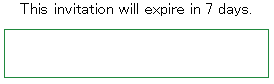
\includegraphics{img/GitHub-invitation.png}
    \caption{GitHub invitation link when it appears empty.}
    \alttext{A blank rectangular box with the text ``This invitation will expire in 7 days'' written above.}
    \label{fig:gh-invitation}
\end{figure}


\subsubsection{Make a new GitHub repository for your notes using the SoM template}

Sign in to your GitHub account, and go to the \href{https://github.com/UoE-School-of-Mathematics/Workflow-Template-Blank}{blank template repository}. Then, click the ``Use this template'' button at the top right of the page. This will create a new repository for you containing the template files.

\begin{figure}[h]
    \centering
    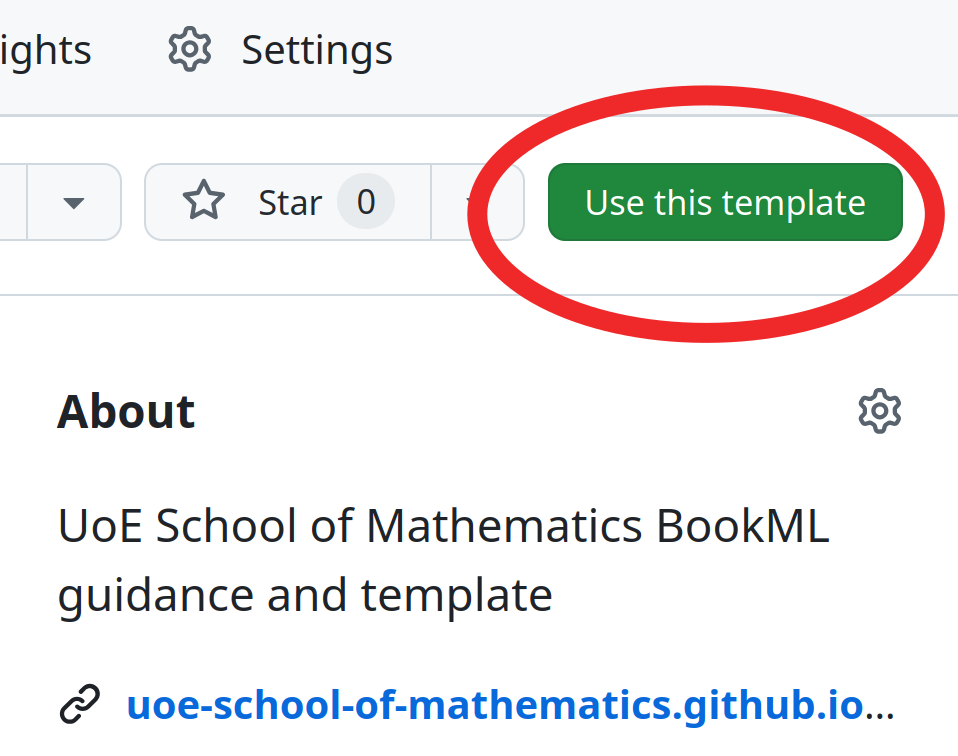
\includegraphics[width=0.5\textwidth]{img/use_template.png}
    \alttext{A screenshot of a webpage showing a green ``Use this template'' button circled in red.}
    \caption{``Use this template'' button is at the top right of the page.}
    \label{fig:use-template}
\end{figure}

The ``Create a new repository'' page has some options:

\begin{itemize}
    \item Keep ``Include all branches'' \textbf{unticked}.
    \item Change ``Owner'' to \textbf{``UoE-School-of-Mathematics''}. This will ensure that your notes are stored in a private repository on GitHub in the UoE School of Mathematics organization\footnote{If you prefer the repository to be owned by your own GitHub account instead, one important difference is that the GitHub Actions minutes needed to perform the HTML conversion in the cloud will be taken from your own GitHub account's quota. The SoM organization has a larger allowance; this is why we encourage you to use it.}.
    \item Choose an appropriate repository name; we recommend that you choose your \textbf{course abbreviation} (e.g. FAC, IMU, IDS, FPM\ldots), or include it in the name.
    \item Make sure ``Visibility'' is \textbf{``Private''}.
\end{itemize}

Finally, click ``Create repository'' and wait at least 3~minutes before moving on. GitHub needs some time to initialise the project.

\subsubsection{Not using Overleaf?}

At this stage, you will have your own copy of the SoM template, as your own repository on GitHub. Steps 2 and 3 below use Overleaf, which makes things easier if you're not familiar with GitHub. However, it's also possible to not use Overleaf at all if you prefer to work locally:

\begin{itemize}
    \item If you are comfortable working with git, you can clone your new repository, and push your changes to GitHub to update the HTML version.
    \item If not, you can also download the files from GitHub (\href{https://docs.github.com/en/get-started/start-your-journey/downloading-files-from-github#downloading-a-repositorys-files}{following these instructions}), extract the .zip, write your notes in that folder, and re-upload any .tex files you have changed directly to GitHub (\href{https://docs.github.com/en/get-started/start-your-journey/uploading-a-project-to-github#step-2-upload-files-to-your-projects-repository}{following these instructions}) every time you want to update the HTML version.
\end{itemize}

In any case, if you do this, you can skip directly to section \ref{ssec:download}.


\subsection{Step 2: Create an Overleaf project linked to your GitHub repository}
\label{ssec:overleaf}

\subsubsection{Link your Overleaf account to your GitHub account}

Visit your \href{https://www.overleaf.com/user/settings}{Overleaf account settings}. Under \textbf{Project Synchronisation}, click \textbf{Link} next to \textbf{GitHub Sync}. Follow the prompts to link Overleaf and GitHub.

\subsubsection{Make an Overleaf project from your GitHub repository}

At this stage, you should have a GitHub repository created from the SoM template. In Overleaf, create a new project, ensuring you choose \textbf{Import from GitHub}. Then, choose \textbf{Import to Overleaf} for the repository you created previously.

\begin{figure}[h]
    \centering
    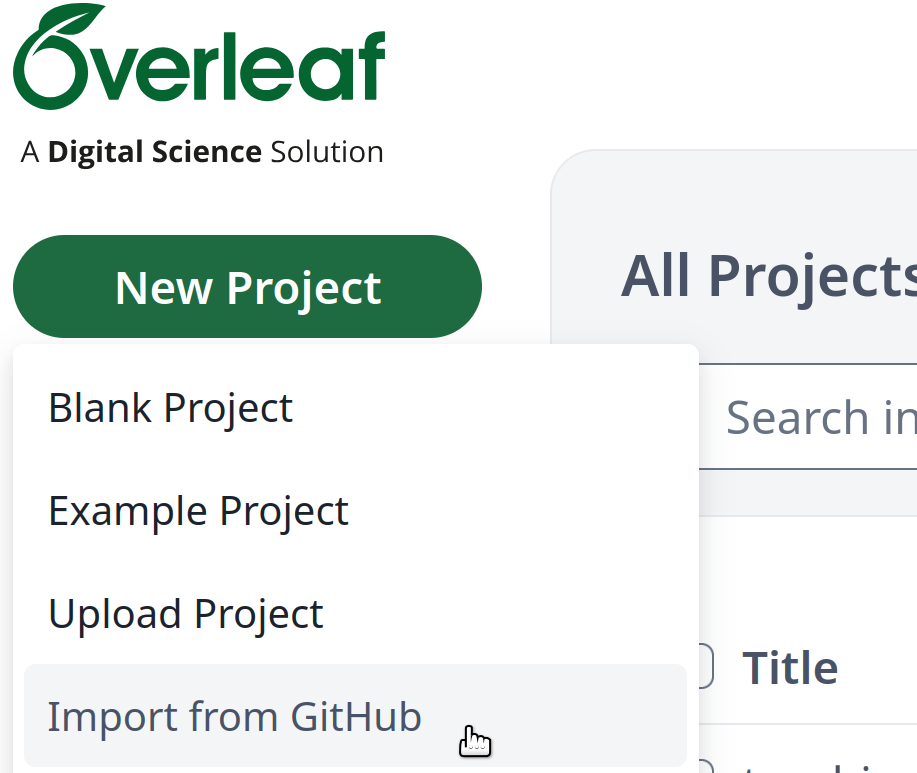
\includegraphics[width=0.5\textwidth]{img/overleaf_new.png}
    \caption{Choose ``Import from GitHub'' when creating the new project.}
    \alttext{A screenshot of the Overleaf ``New project'' options, showing ``Import from GitHub'' selected by the user.}
    \label{fig:gh-overleaf-new}
\end{figure}

Once this is complete, you should have a new Overleaf project containing the template files.


\subsection{Step 3: Write your notes in Overleaf and sync with GitHub}
\label{ssec:sync}

Now you can work on your notes just like with any other Overleaf project.

Whenever you want to publish changes to the HTML version, you need to push the changes to your GitHub repository. To do this, in Overleaf, click \textbf{Menu} (top left) and then choose \textbf{GitHub} under the \textbf{Sync} menu.

\begin{figure}[h]
    \centering
    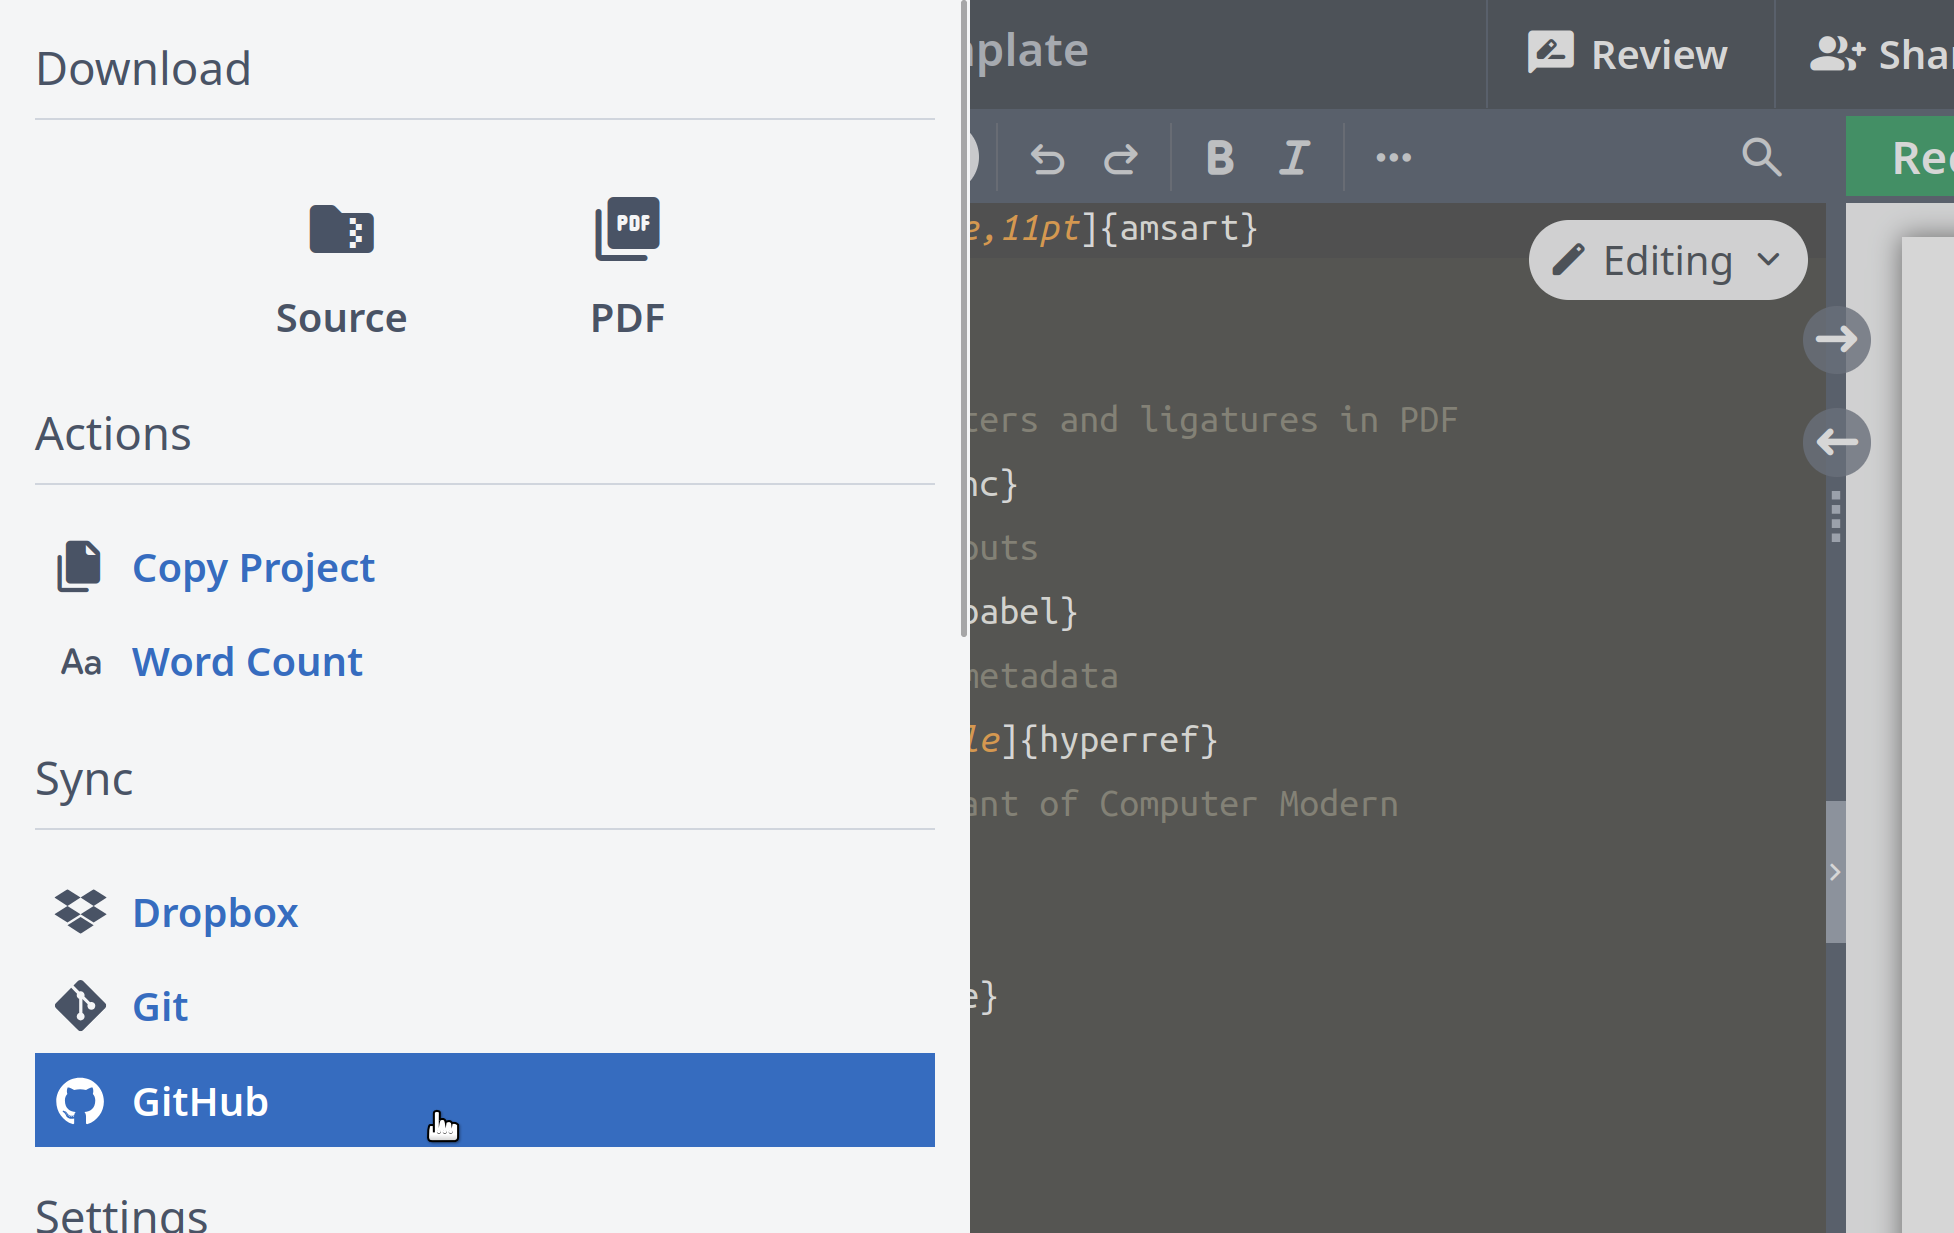
\includegraphics[width=0.6\textwidth]{img/overleaf_sync.png}
    \caption{The ``GitHub'' option in the Overleaf top-left menu.}
    \alttext{A screenshot of the Overleaf menu bar, showing ``GitHub'' selected by the user.}
    \label{fig:gh-overleaf-sync}
\end{figure}

Click \textbf{Push Overleaf changes to GitHub}, enter a description of the changes you have made (optional) and then click \textbf{Sync}.

\subsection{Step 4: Download the generated HTML version of your notes from GitHub as a SCORM package, and upload it to Learn}
\label{ssec:download}

Every time you sync new changes to GitHub, the HTML notes will recompile automatically (this takes a few minutes). Visit your GitHub repository; a green check mark above your files indicates that this has completed. Scroll to ``Releases'' in the right-side menu, and click on the \texttt{SCORM.main.zip} file\footnote{The word \texttt{main} may be replaced by the name of any .tex file with \texttt{documentclass} in it. If you have multiple separate documents in your project, you will get multiple SCORM files to upload on Learn separately.}. This will download a zip file containing the HTML version of your notes.


\subsubsection{Upload the SCORM file}
\label{ssec:scorm}

\begin{itemize}
    \item On your Learn page, create a new content item.
    \item Choose the ``SCORM package'' option.
    \item Upload the file \verb|SCORM.main.zip|.
    \item Once it's uploaded, untick the ``Mark SCORM'' checkbox, and click ``Save''.
\end{itemize}

\begin{figure}[h!]
    \centering
    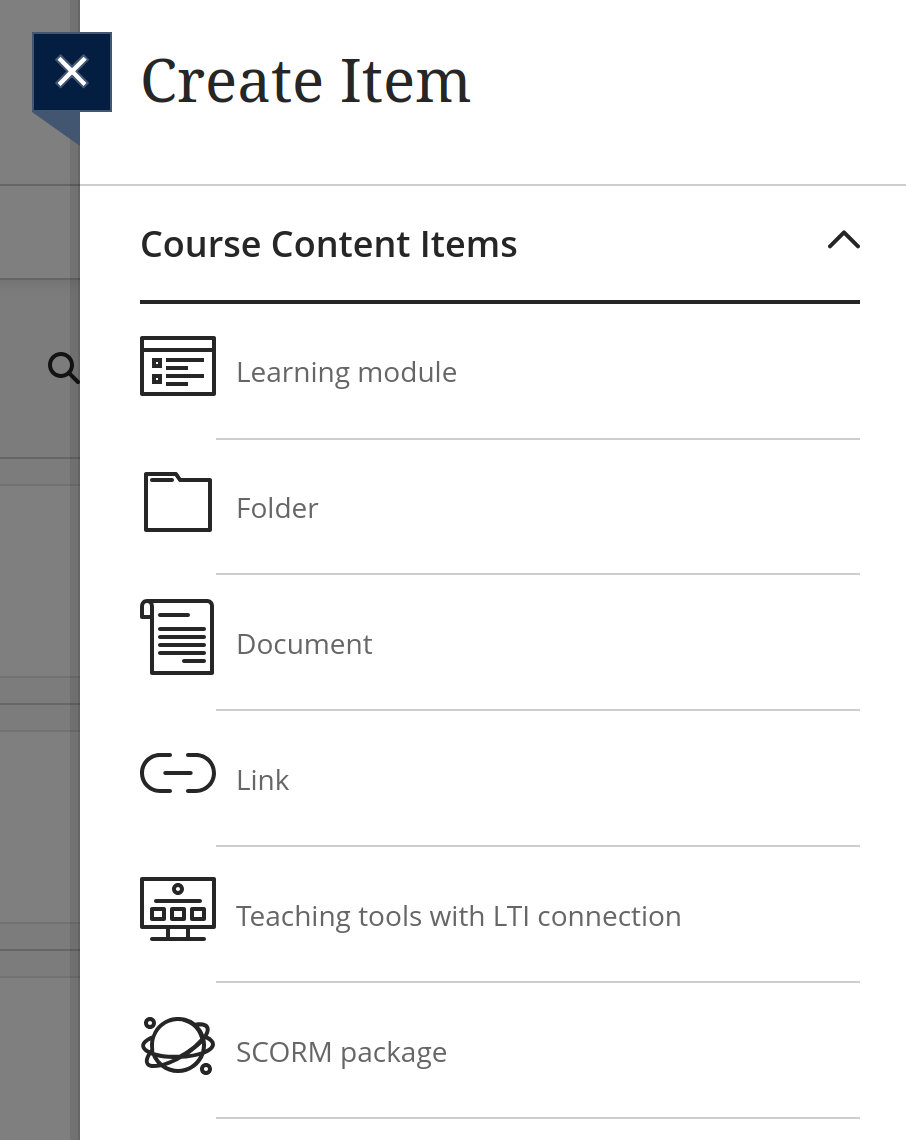
\includegraphics[width=0.5\textwidth]{img/scorm.png}
    \caption{The ``SCORM package'' option on Learn Ultra.}
    \alttext{A screenshot of the ``Create content'' menu on Learn Ultra showing different options. The last option is ``SCORM package''.}
    \label{fig:scorm}
\end{figure}


\subsection{Step 5 (optional): Publish your notes as a public website}
\label{ssec:pub}

Additionally, or alternatively, you can publish your notes as a \textbf{public website} using GitHub Pages. The advantage of doing this, is that this is all already automated; so there is no need for you to manually update your published site every time you update your notes (as you need to do when uploading to Learn). Instead, you can simply add a link to your published website on your Learn page, and this will always point to the most up-to-date version of your notes.

Your site is already built automatically by using the GitHub template, but it's not published by default. To set up a publicly-accessible website with your HTML notes, first visit your repository on GitHub. In the top menu, click \textbf{Settings}, then \textbf{Pages} in the left menu.

Under \textbf{Build and deployment}, look for the \textbf{Branch} option. From the \textbf{Select branch} option, choose \texttt{gh-pages} and \textbf{Select folder} \texttt{/docs}.

\begin{figure}[h]
    \centering
    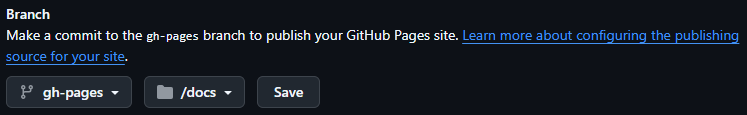
\includegraphics[width=\columnwidth]{img/GitHub-Pages.png}
    \caption{Select the \texttt{gh-pages} branch and the \texttt{/docs} folder.}
    \alttext{A screenshot of a section of the ``Settings'' page. The text reads ``Branch: Make a commit to the gh-pages branch to publish your GitHub Pages site.'' Two drop-down menus and a ``Save'' button are below. The first drop-down menu shows the option ``gh-pages'' was picked. The second shows the option ``/docs''.}
    \label{fig:gh-pages}
\end{figure}

Wait 1~minute then refresh the page. You should now see a link to the publicly-available site hosting your HTML notes. This includes the URL that you should use to share your notes with students.

\begin{figure}[h]
    \centering
    
\includegraphics[width=\columnwidth]{img/GitHub-site-link.png}
    \caption{The link to your course site.}
    \alttext{A screenshot of a section of the ``Settings'' page. The text reads: ``Your site is live at https://uoe-school-of-mathematics.github.io/ohagan_demo/'', then ``Last deployed by sohagan1 last month''. There is a ``Visit site'' button on the right.}
    \label{fig:gh-site-link}
\end{figure}

Behind the scenes, GitHub will now automatically rebuild your HTML notes and update the public website every time you synchronise changes with GitHub. This was a one-time setup; you don't need to interact directly with GitHub again.

\subsubsection*{Copyright and license}
\label{ssec:pub:license}

As per UK law, as explained in \href{https://library.ed.ac.uk/library-help/copyright/copyright-teaching}{University guidance}, the University ``is the first owner of the rights of any work made in the course of your employment'', and this applies to teaching materials. By default, this is attributed at the bottom of the index page of your published site.

The University also has an \href{https://open.ed.ac.uk/how-to-guides/}{Open Educational Resources policy and guidance}; we encourage you to consider publishing your course materials as an open educational resource (and change the copyright notice accordingly).


\subsection{Video Guidance}
\iflatexml
Below is a recording of a demo session showing the cloud based workflow. 
\bmlRawHTML{
    <iframe id="kaltura\_player"
        type="text/javascript"
        src="https://cdnapisec.kaltura.com/p/2010292/embedPlaykitJs/uiconf\_id/55171522?iframeembed=true\&entry\_id=1\_zypgaqqb"
        style="width: 608px;height: 402px;border: 0;"
        allowfullscreen=""
        webkitallowfullscreen=""
        mozAllowFullScreen=""
        allow="autoplay *; fullscreen *; encrypted-media *"
        sandbox="allow-forms; allow-same-origin; allow-scripts; allow-top-navigation; allow-pointer-lock; allow-popups; allow-modals; allow-orientation-lock; allow-popups-to-escape-sandbox; allow-presentation; allow-top-navigation-by-user-activation"
        title="Kaltura Player">
    </iframe>}
\else
A \href{https://media.ed.ac.uk/media/BookML+LaTeX+to+HTML+Demo+%28recording%29/1_zypgaqqb}{recording of a demo session}
showing the cloud based workflow can be found on media hopper.
\fi


\section{Local workflow}

Another way to create and maintain HTML course materials is to convert your notes locally on your machine. To do this, you will need to either install Docker, or directly install BookML and its dependencies. We give detailed instructions for the Docker workflow, as this is generally easier to set up and use.

\subsection{Using Docker}
\label{ssec:docker}

To run BookML, we can use a Docker container --- a lightweight, portable unit that packages an application and all its dependencies, ensuring that it runs consistently across different environments. This removes the need to download software and maintain dependencies on your computer.

Importantly for us: there is a \href{https://github.com/vlmantova/bookml/pkgs/container/bookml}{Docker image available for BookML}, which is ready-to-use and contains everything we need.

To use it, we can use Docker Desktop, which is available for Windows and Mac, or Docker Engine, which is available for Linux. An open-source alternative (compatible with Docker) is Podman, which is available for Windows, Mac, and Linux. In any case, the key steps are:

\begin{enumerate}
    \item Setup (just once): install Docker or Podman, and download the Docker image.
    \item Convert: run a single command in the folder with your \verb|.tex| files.
\end{enumerate}

Both Docker and Podman allow us to use either the command line or a graphical interface. If you don't know which one to choose, just pick one and try it!

\noindent \textbf{Notes: }
\begin{itemize}
    \item If you have a managed Windows machine, Docker Desktop is available from the software centre. This is a slightly complicated process, 
    see Appendix \ref{app:a} for instructions. It may be simpler to request `Make Me Admin' and install from the internet.
    If you wish to use Podman, you will need to request `Make Me Admin'.
    \href{https://www.ed.ac.uk/information-services/computing/desktop-personal/supported/windows-10/makemeadmin}{Guidance on `Make Me Admin'}.
    \item The Learning Technology team will be able to assist you with installing Docker or Podman --- email \verb|lt@maths.ed.ac.uk| to ask for help.
\end{itemize}

\subsubsection{Setup (first-time only)}
\label{sssec:setup}

\paragraph{Option 1 - to set up Docker:}

\begin{enumerate}
    \item
        \begin{itemize}
            \item \textbf{Windows/MacOS/Linux:} \href{https://docs.docker.com/desktop/install/windows-install/}{Download Docker Desktop from \textbf{this} link} or the Software Centre, and install as instructed by the interface. Launch Docker Desktop. 
There are versions of the download file of Docker Desktop which cause an error. Ensure you are downloading the version that is listed in the documentation.
            \item \textbf{Alternatively for Linux only:} Download and install Docker Engine, following \href{https://docs.docker.com/engine/install/}{the instructions for your distribution}.
        \end{itemize}
    \item Launch a terminal (use \verb|cmd.exe| on Windows), and run the command:\\
        \verb|docker pull ghcr.io/vlmantova/bookml:latest|\\
        This will download the Docker image to your machine.
\end{enumerate}

\paragraph{Option 2 - to \href{https://podman.io/docs/installation}{set up Podman}:}

Note that this requires ``Make Me Admin'' on Windows managed machines.

\begin{enumerate}
    \item \href{https://podman.io/}{Download Podman Desktop from here} and install as instructed by the interface. 
    \item Podman desktop will open, and you will be asked to setup.
    Click the `Setup' button and follow through the instructions 
    that follow. When prompted, select `Yes', and then `Install'. 
    \item Once fully installed, we can download the image. To do this, open the `Images' tab
        (the 4th option on the left-hand side of the screen) and click \verb|Pull| on the top right of the screen, then enter \verb|ghcr.io/vlmantova/bookml:latest| and click ``Pull image''. 
\end{enumerate}

\subsubsection{Conversion}
\label{sssec:conversion}

Before you start, for better results, add \verb|\usepackage{bookml/bookml}| to the preamble of your \verb|.tex| file(s) (after the \textbackslash\verb| documentclass{...}| command). This is not necessary if you are using the \href{https://github.com/UoE-School-of-Mathematics/Workflow-Template-Blank/releases}{template provided here by the School of Mathematics} (download and extract ``Source code (zip)'').

Note that if you use Overleaf, the \verb|bookml/bookml| package will cause an error, unless you also add the \verb|bookml| folder to your project (found in \verb|release.zip| on the \href{https://github.com/vlmantova/bookml/releases}{BookML repository}).

\paragraph{Option (a) - using the command line:}

\begin{enumerate}
    \item Start a terminal in the directory containing your \verb|.tex| file(s). (Use \verb|cmd.exe| in Windows.)
    \item Run the command:\\
        \verb|{software} run -t -v .:/source ghcr.io/vlmantova/bookml:latest|\\
        (replace \verb|{software}| with \verb|docker| or \verb|podman|).
\end{enumerate}

\paragraph{Option (b) - using the graphical interface:}

\begin{enumerate}
    \item In Docker/Podman Desktop, click on the `Images' tab, and you will see the image you have just downloaded. Click the `Play' button (Figure~\ref{fig:docker_desktop_run}).
    \item Under ``Volumes'', specify the ``Host path'' to be the path to your folder, and the ``Container path'' to be \verb|/source|. (In Docker Desktop, this is under ``Optional settings'' -- see Figure~\ref{fig:docker_desktop_path}.)
    % \item In `Optional settings', under `Volumes', in the left box called \verb|Host Path|, copy the path to your folder, or click the three dots to navigate to the folder. In the right box labelled `Container Path', type \verb|/source|.
    \item Click `Run' (Docker) or `Start Container' (Podman) to produce the PDF and HTML outputs.
\end{enumerate}

\begin{figure}[h!]
    \centering
    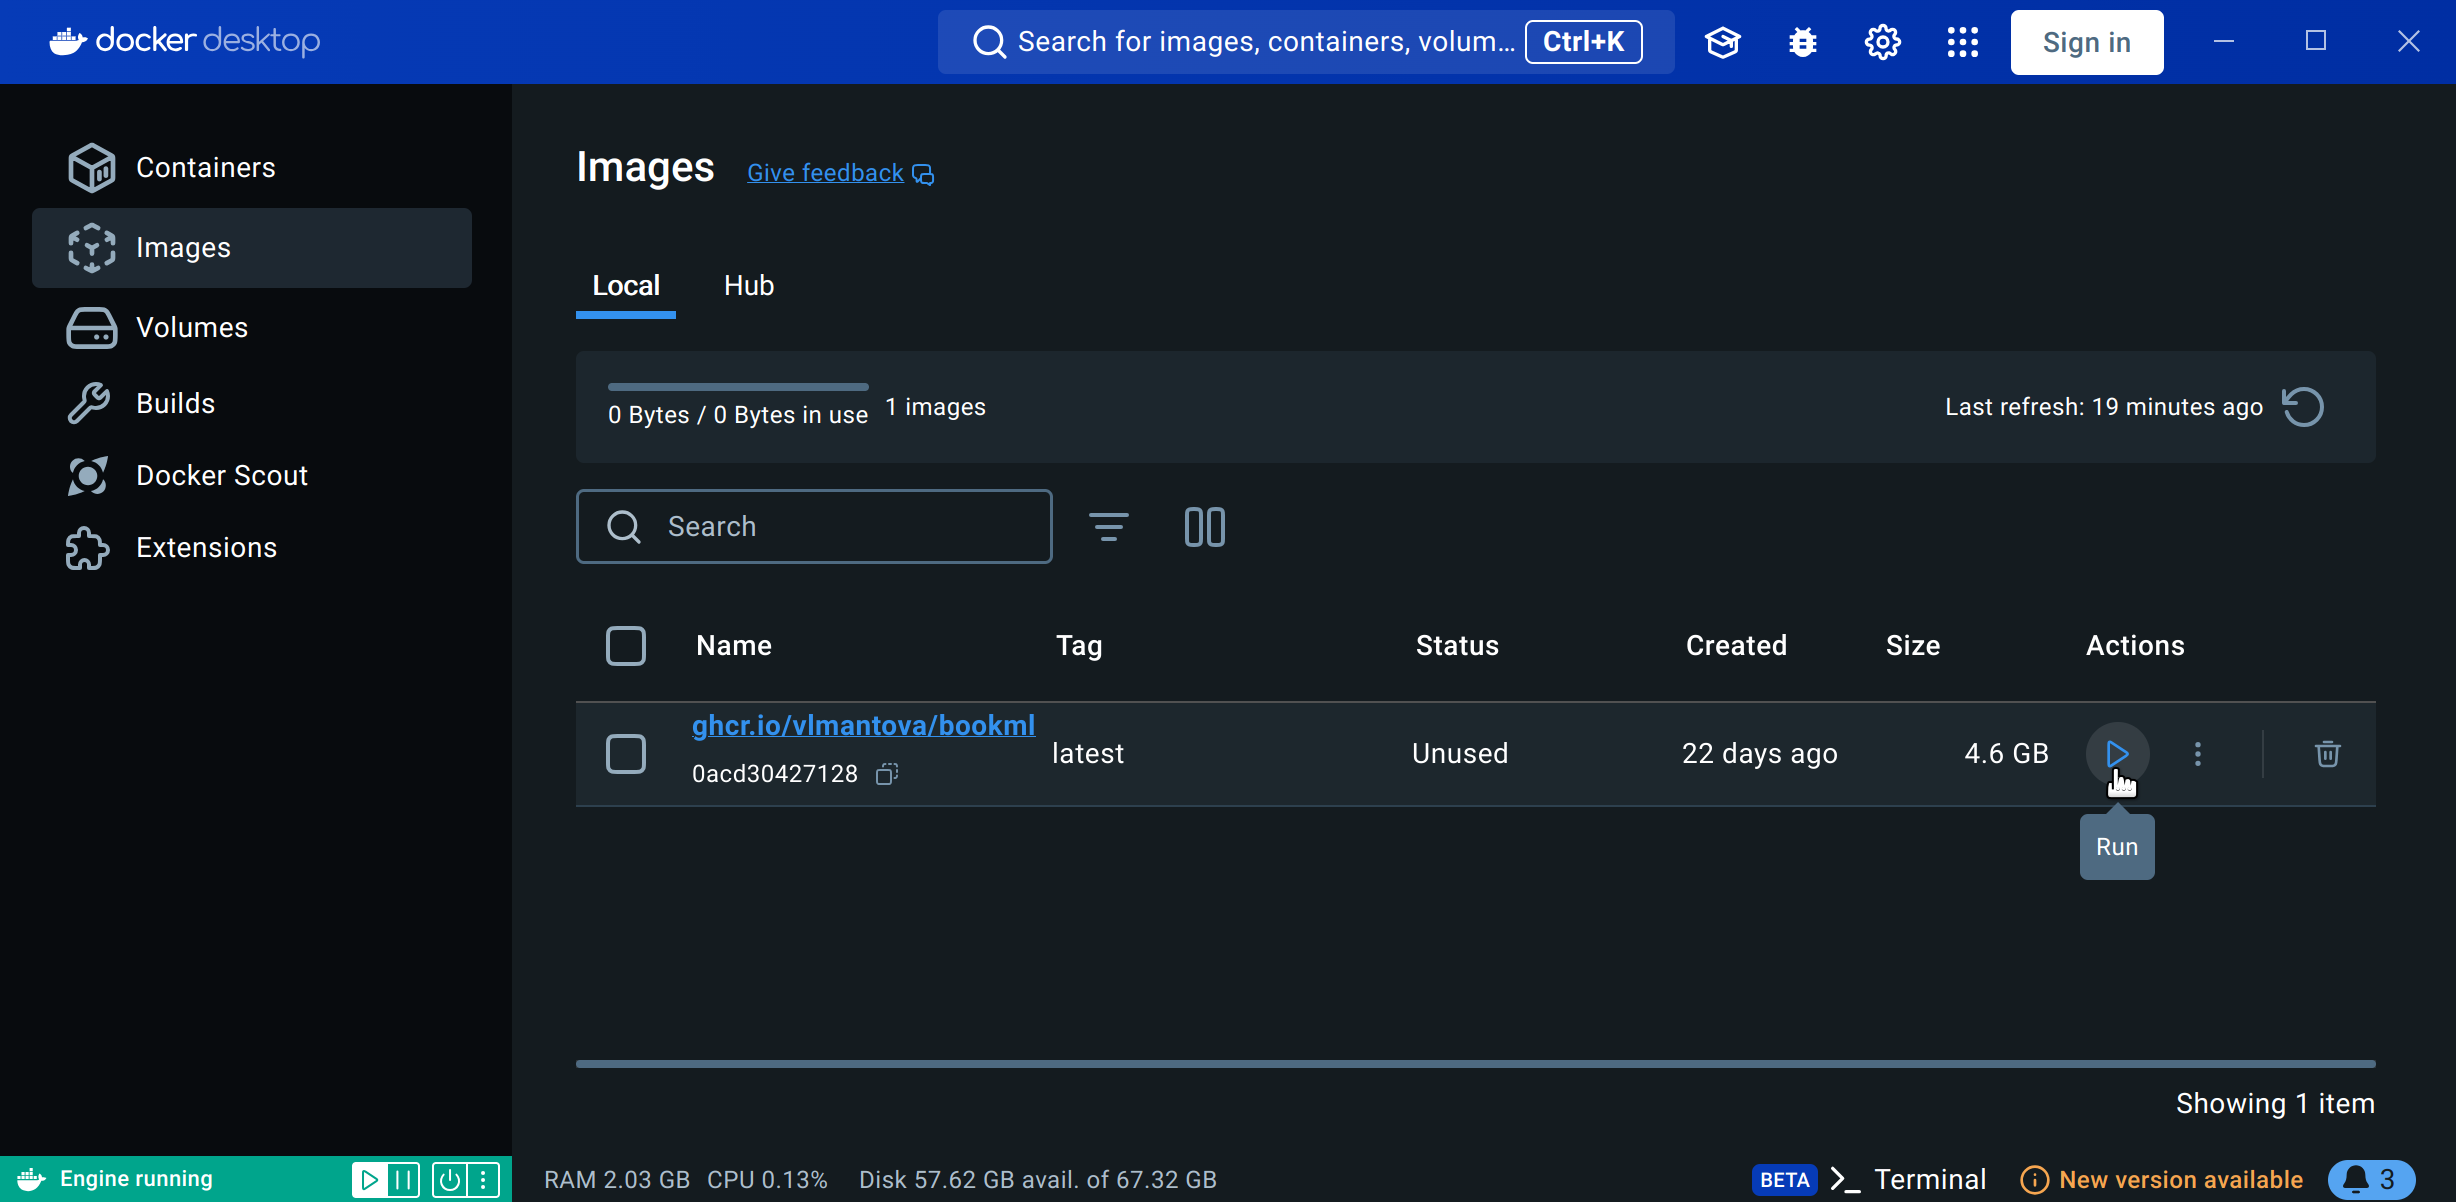
\includegraphics[width=\textwidth]{img/docker_desktop_run.png}
    \caption{Step 1: click the `play' button to run the command.}
    \alttext{A screenshot of Docker Desktop, with the cursor placed on the ``Run'' button.}
    \label{fig:docker_desktop_run}
\end{figure}

\begin{figure}[h!]
    \centering
    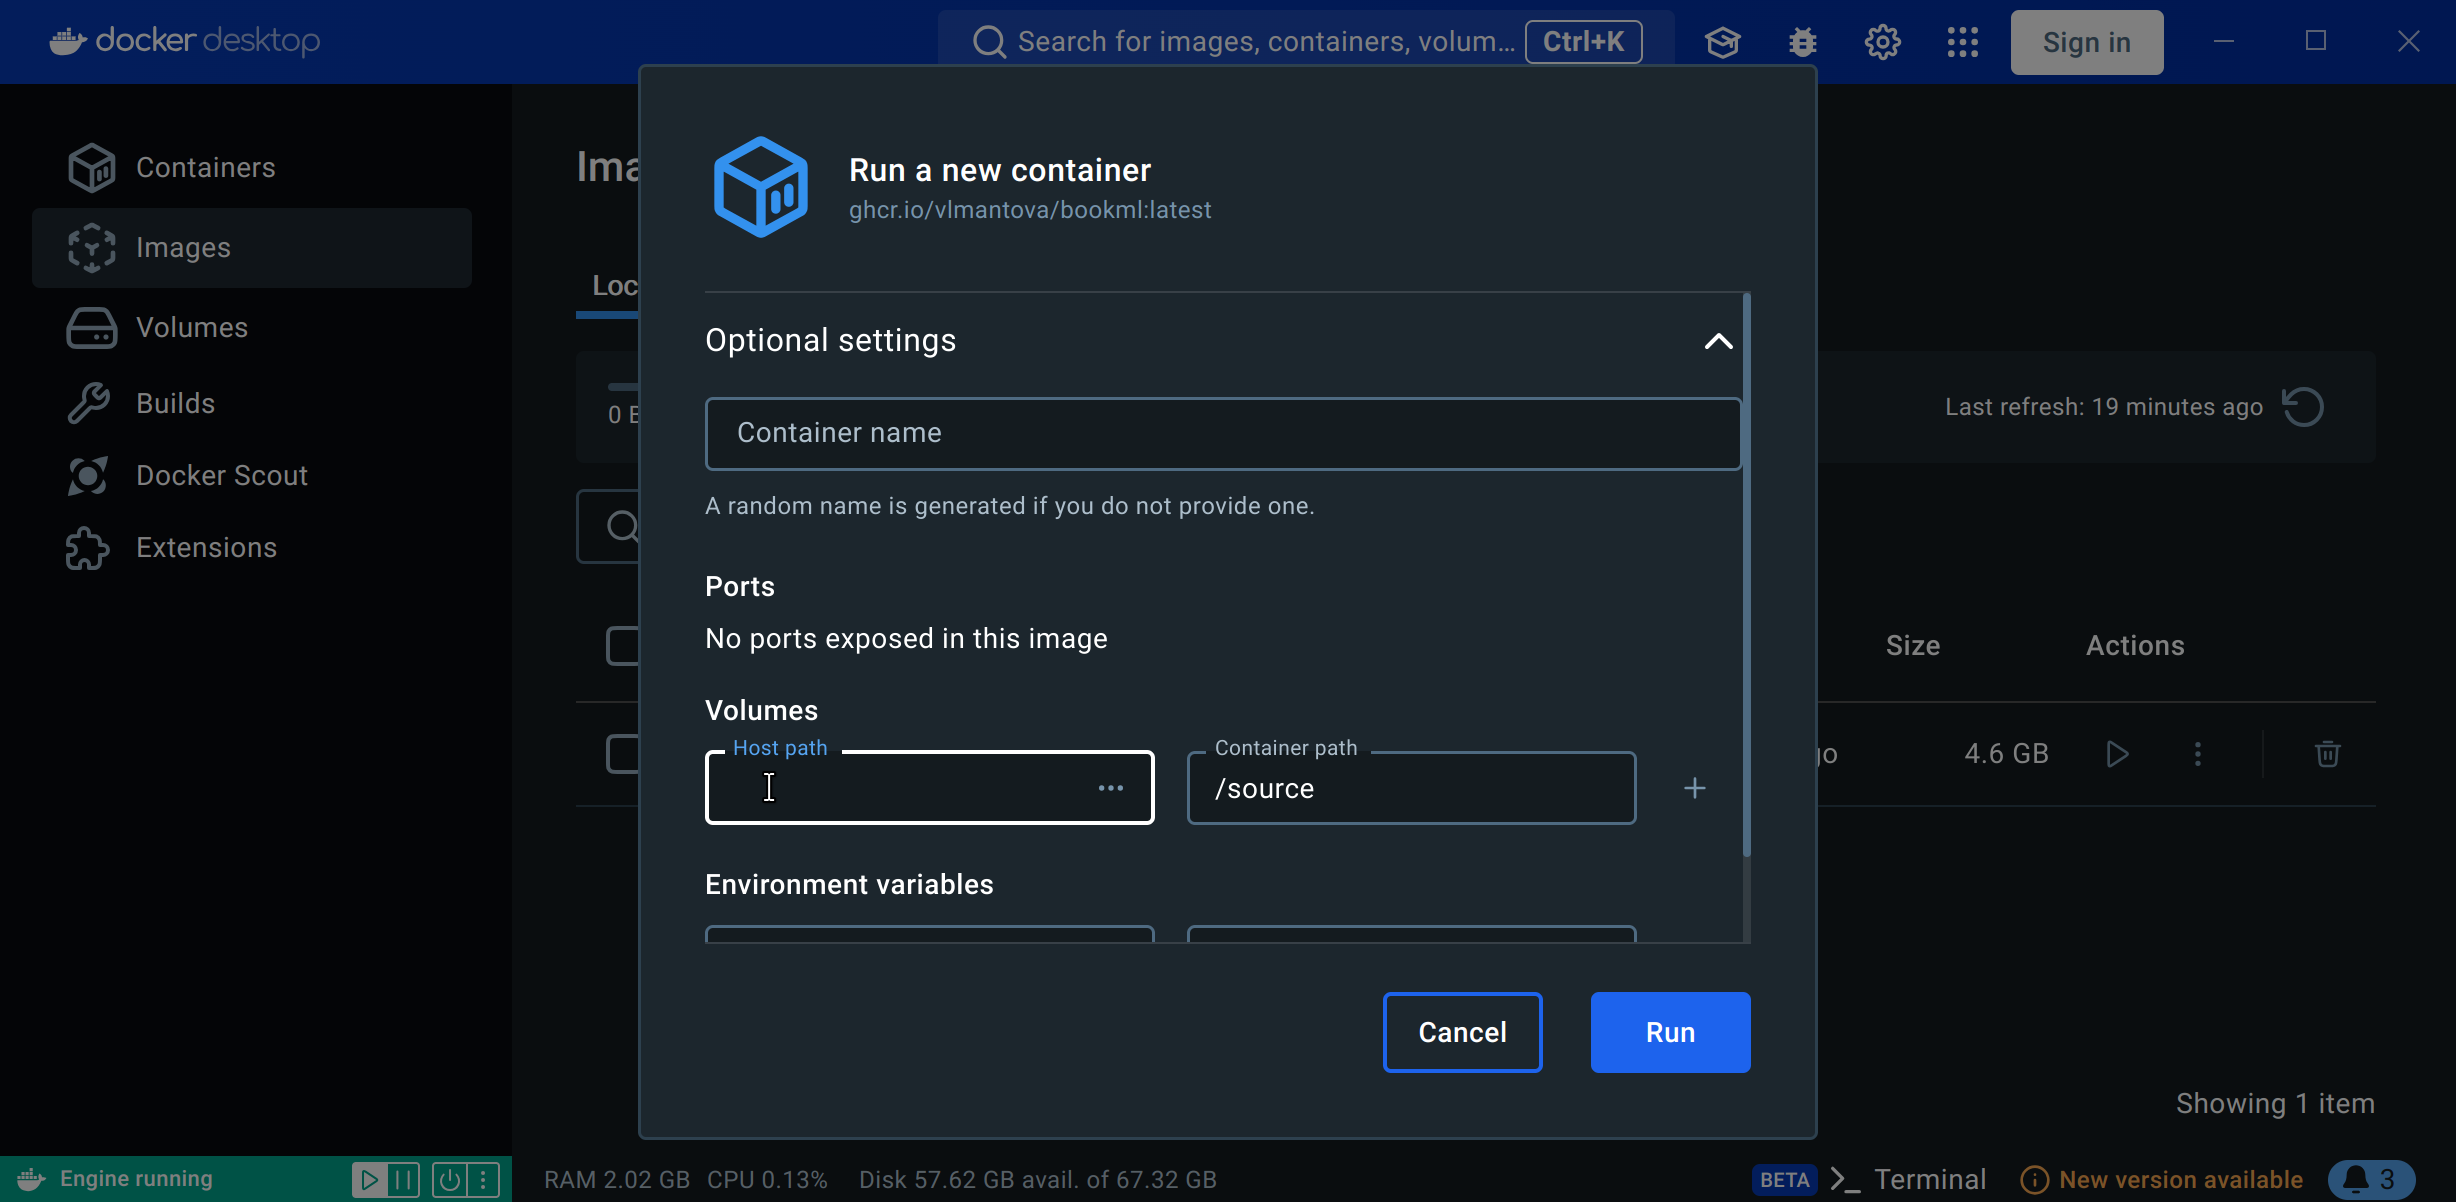
\includegraphics[width=\textwidth]{img/docker_desktop_path.png}
    \caption{Step 2: give Docker the path to your folder.}
    \alttext{A screenshot of Docker Desktop, showing where to input the folder path.}
    \label{fig:docker_desktop_path}
\end{figure}

\subsection{Installing BookML and dependencies manually}
\label{ssec:install}

If you prefer to install the necessary packages and dependencies to your machine instead of using Docker, instructions are given in the \href{https://vlmantova.github.io/bookmlleeds/#S1}{BookML documentation} for the installation and the conversion to HTML.


\subsection{Sharing with students}
\label{ssec:local:share}

Running BookML will produce PDF files (with \verb|pdflatex|), as well as \verb|.zip| files containing the HTML versions of your \verb|.tex| files, which can be uploaded directly to Learn. The output (both PDF and HTML) will be found in the same folder as your \verb|.tex| files.
Upload \verb|SCORM.yourfile.zip| directly to Learn as described in \ref{ssec:scorm}.

The \verb|yourfile.zip| (without the \verb|SCORM|) files contain a standalone HTML site, which you may also wish to publish yourself if you are comfortable doing so (e.g. on your SoM user domain). See \ref{ssec:pub:license} for related copyright information. However, only the \verb|SCORM| versions are fully compatible with Learn, so please use these if you plan to upload your materials to Learn.


\subsection{Learning Technology Mailbox}
\label{ssec:lt}

If you would rather, you can also email \verb|lt@maths.ed.ac.uk| with a .zip of the folder containing all the source files for your course materials (everything needed for your .tex files to compile normally). The Learning Technology team will perform the conversion, and email you back with a .zip file containing the HTML version of your course materials; optionally, they can also upload it to your Learn page. If they spot anything which didn't convert well, they will let you know.


\section{FAQs}
\label{sec:FAQ}

\noindent\textbf{Q: Error: \texttt{Warning: no .tex files with \textbackslash{}documentclass found in this directory}}
\begin{ans}
    The software cannot reach your files, this may be due to running the software in the wrong place, permissions, or a remote directory. 
    Double check your file path, and try moving the files to a local directory and try again.
\end{ans}

\noindent\textbf{Q: Why aren't my files converting at all, there is not an error, BookML simply states there are no files to convert.} 
\begin{ans}
    This is likely due to the fact that the software cannot reach your files. This can be because your files are in a folder, or that your files have \href{https://stackoverflow.com/questions/1976007/what-characters-are-forbidden-in-windows-and-linux-directory-names}{forbidden file characters} or a space.
\end{ans}

\noindent\textbf{Q: The conversion process is taking a very long time.}
\begin{ans}
    The conversion process can take a while, especially for larger documents --- but if it's 30 minutes or more, then please flag this. Note that, if you are using a local installation (not Docker), there are some known issues related to this:
    \begin{itemize}
        \item There is a \href{https://github.com/brucemiller/LaTeXML/issues/2268}{known issue} with the package \verb|expl3| when used with TeXlive 2022 and older which can cause the conversion to take longer.
        \item There is a known issue with the ``postprocessing XSLT'' stage taking several minutes (instead of seconds) on Ubuntu 22.04.
    \end{itemize}
\end{ans}
 
\noindent\textbf{Q: Will my .tex files be converted if I comment out} \verb|\|\verb|documentclass|? 
\begin{ans}
    Yes, and it may cause errors. For files which you don't want to be converted standalone (e.g. files which are \verb|\input|ted into another file), delete the \verb|\|\verb|documentclass| command entirely or move them into a folder.
\end{ans}


\section{Other accessibility information}
\label{sec:otheraccessibility}

This is not the whole picture. There are other things to consider when creating accessible documents that is not handled by materials being in HTML. Additionally, there are other alternatives to a \LaTeX to HTML conversion.

\subsection{Other considerations}
\label{ssec:otheraccessibility}

\begin{itemize}
    \item \textbf{Images:} Ensure that all images have \textit{quality} alternative text. This is not done automatically by BookML, so you will need to add this manually. Information on how to add alt text is in the demo portion of this document (see Section~\ref{demo:fig}), with information about images.
    \item \textbf{Links:} Ensure that all link text is accessible.
    \item \textbf{Use of colour:} Colour should not be used exclusively to communicate information. This is often missed in graphs and charts. For example, portions of a pie chart should be directly labelled, or the legend should be additionally texture-based.
\end{itemize}

\subsection{Alternatives to BookML}
\label{ssec:alternatives}

If you are not strongly attached to using \LaTeX, then instead of using BookML, you can create course materials in accessible formats using \href{https://www.markdownguide.org/basic-syntax/}{the Markdown language}. Software such as \href{https://bookdown.org/}{Bookdown} or \href{https://quarto.org/}{Quarto} offer Markdown support and extended features, and allow you to produce materials in a range of formats (including PDF, HTML, computational notebooks\ldots) directly from Markdown source.

% With these formats you may wish to upload the produced HTML files to Learn. See instructions in Section \ref{appb:zip} for how to upload a zip file to Learn.

% \appendix
% \section{Docker from software centre}
% \label{app:a}
% This method is more complicated than the Docker Desktop download from the internet, but avoids need of admin privileges.
% \begin{enumerate}
    % \item Open the Software Centre and search for Docker Desktop.
    % \item Click on the Docker Desktop icon and click `Install'.
    % \item This download may give the message it has failed, click retry.
    % \item Repeat this a few times, between each download type `docker' into a terminal window and press enter.
     % If docker is installed, the terminal will return a long message about docker commands. If it is not, it will not recognise the command.
    % \item Eventually, the download will prompt a restart. Allow this.
    % \item At this point, leave the machine for an extended time, potentially overnight. 
    % \item After this time, open a terminal window and type `docker' and press enter. 
    % \item Install once again, and the download should be successful. Check using the terminal.
% \end{enumerate}
